\clearpage
\section{Period of a relaxation oscillation}
\subsection{Lienard variable}
the lienard variable 
\begin{equation}
    y = \frac{\dot{x}}{k}+F(x)
\end{equation}
so 
\begin{equation}
    \dot{x} = k\ins{y-F(x)}
\end{equation}
and 
\begin{equation}
    \dot{y} = \frac{\ddot{x}}{k}+F'(x)\dot{x}=\frac{\ddot{x}+k\ins{x^2-4}\dot{x}}{k}
\end{equation}
inserting the original equation 
\begin{equation}
    \dot{y} = \frac{1-x}{k}
\end{equation}
so the system is 
\begin{align}
    \dot{x} = k\ins{y-\frac{x^3}{3}+4x} && \dot{y} = \frac{1-x}{k}
\end{align}
and we can notice that \(x\) is fast and \(y\) is slow.
\subsection{slow parts}
The stability if the fast part is determined by 
\begin{equation}
    \pdv{\dot{x}}{x}=-kF'(x)=-k\ins{x^2-4}
\end{equation}
which is attracting when 
\begin{equation}
    F'(x)=x^2-4>0
\end{equation}
i.e 
\begin{equation}
    x<-2\quad \text{or}\quad x>2
\end{equation}
so we look at \(x=\pm2\) with 
\begin{equation}
    F(2) = -\frac{16}{3} \quad F(-2)=\frac{16}{3}
\end{equation}
finding the other points at which we get these values
\begin{equation}
    x^3-12x-16=0 \implies \ins{x-4}\ins{x+2}^2
\end{equation}
so the trajectory jumps
\begin{equation}
    \ins{-2,16/3} \rightarrow \ins{4,16/3}
\end{equation}
similarly 
\begin{equation}
    \ins{2,-16/3} \rightarrow \ins{-4,-16/3}
\end{equation}
so the slow parts are 
\begin{equation}
    \ins{-4,-16/3}\rightarrow\ins{-2,16/3} \qquad \ins{4,16/3}\rightarrow\ins{2,-16/3}
\end{equation}
\begin{figure}[H]
    \centering 
    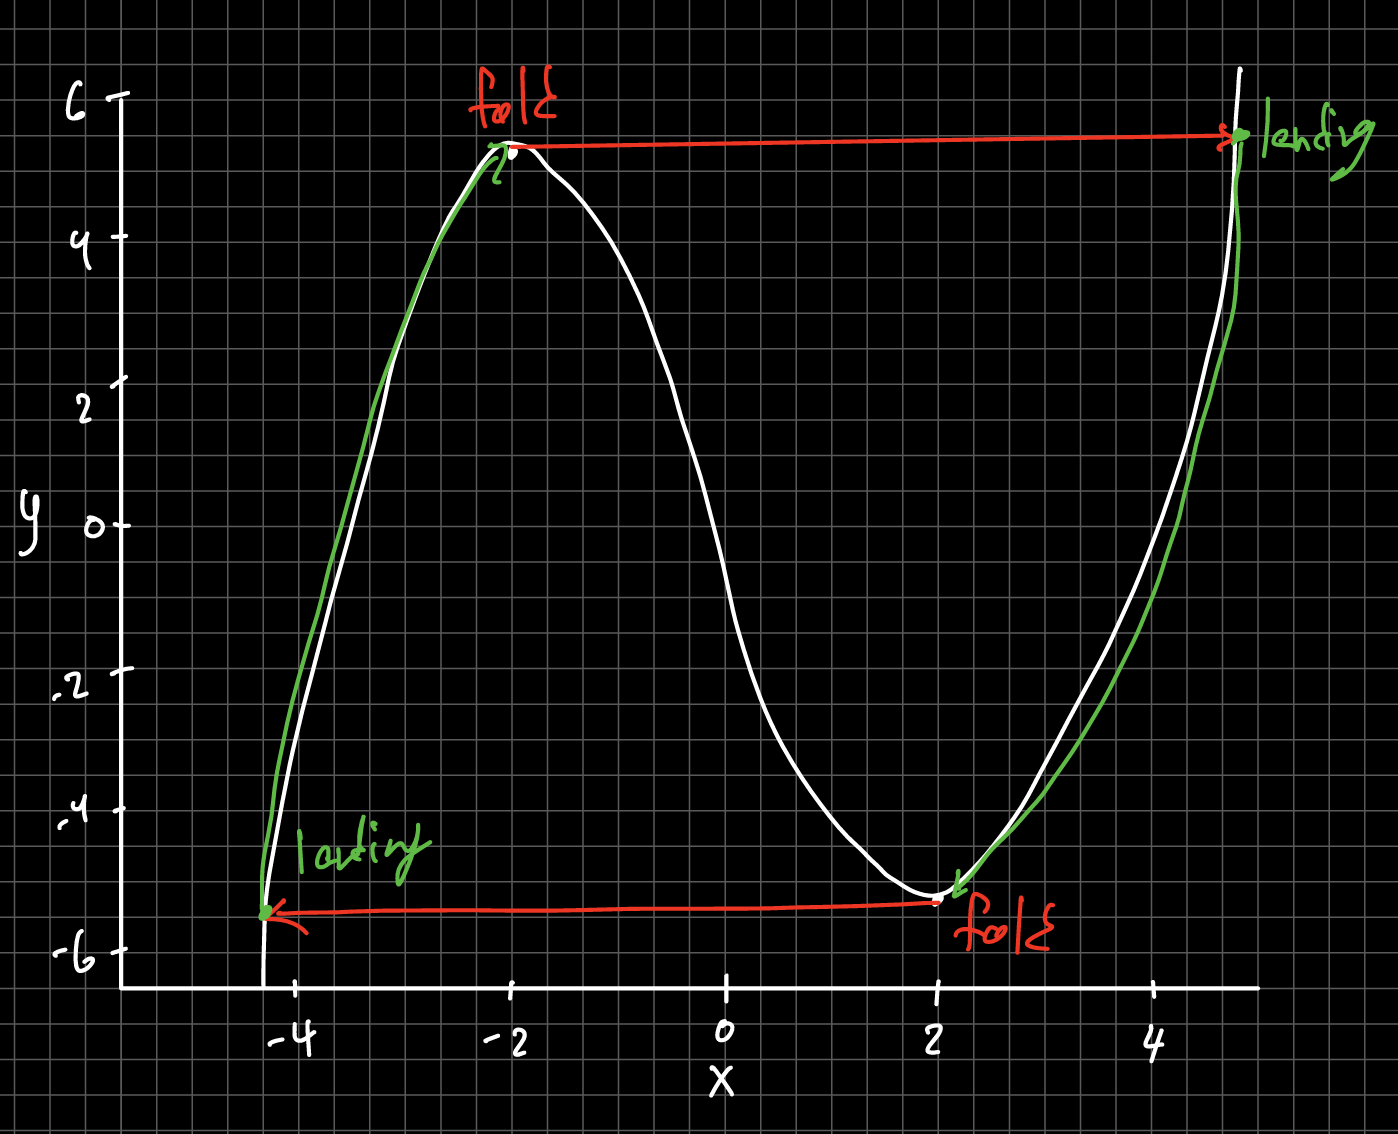
\includegraphics[width=0.75\textwidth]{fig4.png}
\end{figure}
\subsection{period}
on a slow branch 
\begin{equation}
    y \sim F(x)
\end{equation}
so 
\begin{equation}
    \dot{y} \sim F'(x)\dot{x}=\ins{x^2-4}\dot{x}
\end{equation}
using \(\dot{y} = \frac{1-x}{k}\)
\begin{equation}
    \dot{x}=\frac{1-x}{k\ins{x^2-4}}
\end{equation}
so
\begin{equation}
    \dd{t} = k\frac{x^2-4}{1-x}\dd{x}
\end{equation}
so 
\begin{equation}
    T = k\int_{a}^{b}\frac{x^2-4}{1-x} = \left.k\ins{-\frac{x^2}{2}-x+3\ln\abs{x-1}}\right|_a^b
\end{equation}
on the right branch x goes from 4 to 2 so 
\begin{equation}
    T_R = \left.k\ins{-\frac{x^2}{2}-x+3\ln\abs{x-1}}\right|_4^2 = k\ins{8-3\ln3}
\end{equation}
and on the left x goes from -4 to -2
\begin{equation}
    T_L = \left.k\ins{-\frac{x^2}{2}-x+3\ln\abs{x-1}}\right|_{-4}^{-2} = k\ins{4-3\ln\frac{5}{3}}
\end{equation}
so the period time is approximately
\begin{equation}
    T = T_R + T_L = k\ins{8-3\ln3}+k\ins{4-3\ln\frac{5}{3}}=k\ins{12-3\ln5}
\end{equation}